\iffalse
\let\negmedspace\undefined
\let\negthickspace\undefined
\documentclass[journal,12pt,Twocolumn]{IEEEtran}
       \def\inputGnumericTable{}                                 %%
\usepackage{cite}
\usepackage{amsmath,amssymb,amsfonts,amsthm}
\usepackage{algorithmic}
\usepackage{graphicx}
\usepackage{textcomp}
\usepackage{xcolor}
\usepackage{txfonts}
\usepackage{listings}
\usepackage{enumitem}
\usepackage{mathtools}
\usepackage{gensymb}
\usepackage[breaklinks=true]{hyperref}
\usepackage{tkz-euclide} % loads  TikZ and tkz-base
\usepackage{listings}
\usepackage{gvv}

%\usepackage{setspace}
%\usepackage{gensymb}
%\doublespacing
%\singlespacing
%\usepackage{graphicx}
%\usepackage{amssymb}
%\usepackage{relsize}
%\usepackage[cmex10]{amsmath}
%\usepackage{amsthm}
%\interdisplaylinepenalty=2500
%\savesymbol{iint}
%\usepackage{txfonts}
%\restoresymbol{TXF}{iint}
%\usepackage{wasysym}
%\usepackage{amsthm}
%\usepackage{iithtlc}
%\usepackage{mathrsfs}
%\usepackage{txfonts}
%\usepackage{stfloats}
%\usepackage{bm}
%\usepackage{cite}
%\usepackage{cases}
%\usepackage{subfig}
%\usepackage{xtab}
%\usepackage{longtable}
%\usepackage{multirow}
%\usepackage{algorithm}
%\usepackage{algpseudocode}
%\usepackage{enumitem}
%\usepackage{mathtools}
%\usepackage{tikz}
%\usepackage{circuitikz}
%\usepackage{verbatim}
%\usepackage{tfrupee}
%\usepackage{stmaryrd}
%\usetkzobj{all}
    \usepackage{color}                                            %%
    \usepackage{array}                                            %%
    \usepackage{longtable}                                        %%
    \usepackage{calc}                                             %%
    \usepackage{multirow}                                         %%
    \usepackage{hhline}                                           %%
    \usepackage{ifthen}                                           %%
 %optionally (for landscape tables embedded in another document): %%
    \usepackage{lscape}     
%\usepackage{multicol}
%\usepackage{chngcntr}
%\usepackage{enumerate}

%\usepackage{wasysym}
%\documentclass[conference]{IEEEtran}
%\IEEEoverridecommandlockouts
% The preceding line is only needed to identify funding in the first footnote. If that is unneeded, please comment it out.

\newtheorem{theorem}{Theorem}[section]
\newtheorem{problem}{Problem}
\newtheorem{proposition}{Proposition}[section]
\newtheorem{lemma}{Lemma}[section]
\newtheorem{corollary}[theorem]{Corollary}
\newtheorem{example}{Example}[section]
\newtheorem{definition}[problem]{Definition}
%\newtheorem{thm}{Theorem}[section] 
%\newtheorem{defn}[thm]{Definition}
%\newtheorem{algorithm}{Algorithm}[section]
%\newtheorem{cor}{Corollary}
\newcommand{\BEQA}{\begin{eqnarray}}
\newcommand{\EEQA}{\end{eqnarray}}
\newcommand{\define}{\stackrel{\triangle}{=}}
\theoremstyle{remark}
\newtheorem{rem}{Remark}

%\bibliographystyle{ieeetr}
\begin{document}
%

\bibliographystyle{IEEEtran}


\vspace{3cm}

\title{
%	\logo{
GATE-EC2023
%	}
}
\author{ Jay Vikrant EE22BTECH11025
	
	
}	
%\title{
%	\logo{Matrix Analysis through Octave}{\begin{center}\includegraphics[scale=.24]{tlc}\end{center}}{}{HAMDSP}
%}


% paper title
% can use linebreaks \\ within to get better formatting as desired
%\title{Matrix Analysis through Octave}
%
%
% author names and IEEE memberships
% note positions of commas and nonbreaking spaces ( ~ ) LaTeX will not break
% a structure at a ~ so this keeps an author's name from being broken across
% two lines.
% use \thanks{} to gain access to the first footnote area
% a separate \thanks must be used for each paragraph as LaTeX2e's \thanks
% was not built to handle multiple paragraphs
%

%\author{<-this % stops a space
%\thanks{}}
%}
% note the % following the last \IEEEmembership and also \thanks - 
% these prevent an unwanted space from occurring between the last author name
% and the end of the author line. i.e., if you had this:
% 
% \author{....lastname \thanks{...} \thanks{...} }
%                     ^------------^------------^----Do not want these spaces!
%
% a space would be appended to the last name and could cause every name on that
% line to be shifted left slightly. This is one of those "LaTeX things". For
% instance, "\textbf{A} \textbf{B}" will typeset as "A B" not "AB". To get
% "AB" then you have to do: "\textbf{A}\textbf{B}"
% \thanks is no different in this regard, so shield the last } of each \thanks
% that ends a line with a % and do not let a space in before the next \thanks.
% Spaces after \IEEEmembership other than the last one are OK (and needed) as
% you are supposed to have spaces between the names. For what it is worth,
% this is a minor point as most people would not even notice if the said evil
% space somehow managed to creep in.



% The paper headers
%\markboth{Journal of \LaTeX\ Class Files,~Vol.~6, No.~1, January~2007}%
%{Shell \MakeLowercase{\textit{et al.}}: Bare Demo of IEEEtran.cls for Journals}
% The only time the second header will appear is for the odd numbered pages
% after the title page when using the twoside option.
% 
% *** Note that you probably will NOT want to include the author's ***
% *** name in the headers of peer review papers.                   ***
% You can use \ifCLASSOPTIONpeerreview for conditional compilation here if
% you desire.




% If you want to put a publisher's ID mark on the page you can do it like
% this:
%\IEEEpubid{0000--0000/00\$00.00~\copyright~2007 IEEE}
% Remember, if you use this you must call \IEEEpubidadjcol in the second
% column for its text to clear the IEEEpubid mark.



% make the title area
\maketitle

\newpage

%\tableofcontents

\bigskip

\renewcommand{\thefigure}{\theenumi}
\renewcommand{\thetable}{\theenumi}
%\renewcommand{\theequation}{\theenumi}

%\begin{abstract}
%%\boldmath
%In this letter, an algorithm for evaluating the exact analytical bit error rate  (BER)  for the piecewise linear (PL) combiner for  multiple relays is presented. Previous results were available only for upto three relays. The algorithm is unique in the sense that  the actual mathematical expressions, that are prohibitively large, need not be explicitly obtained. The diversity gain due to multiple relays is shown through plots of the analytical BER, well supported by simulations. 
%
%\end{abstract}
% IEEEtran.cls defaults to using nonbold math in the Abstract.
% This preserves the distinction between vectors and scalars. However,
% if the journal you are submitting to favors bold math in the abstract,
% then you can use LaTeX's standard command \boldmath at the very start
% of the abstract to achieve this. Many IEEE journals frown on math
% in the abstract anyway.

% Note that keywords are not normally used for peerreview papers.
%\begin{IEEEkeywords}
%Cooperative diversity, decode and forward, piecewise linear
%\end{IEEEkeywords}



% For peer review papers, you can put extra information on the cover
% page as needed:
% \ifCLASSOPTIONpeerreview
% \begin{center} \bfseries EDICS Category: 3-BBND \end{center}
% \fi
%
% For peerreview papers, this IEEEtran command inserts a page break and
% creates the second title. It will be ignored for other modes.
%\IEEEpeerreviewmaketitle

%\renewcommand{\theequation}{\theenumi}
%\subsection{Problem}

%\section{Chemistry}
%\begin{enumerate}[label=\arabic*.,ref=\thesection.\theenumi]
%\numberwithin{equation}{enumi}
Q)Let $\{X_n\}_{n \geq 1}$ be a sequence of independent and identically distributed random variables with mean 0 and variance 1, all of them defined on the same
probability space. For n=1,2,3,..., let
\begin{align}
Y_n=\frac{1}{n}{\brak{X_1X_2+X_3X_4+...+X_{2n-1}X_{2n}}} 
\end{align}
Then which of the following statements is/are true? 
\begin{enumerate}[label=(\Alph*)]
\item $\{\sqrt{n}Y_n\}_{n \geq 1}$ converges in distribution to a standard normal random variable.
\item $\{Y_n\}_{n \geq 1}$ converges in 2nd mean to 0.
\item $\{Y_n+\frac{1}{n}\}_{n \geq 1}$ converges in probability to 0.
\item $\{X_n\}_{n \geq 1}$ converges almost surely to 0.
\end{enumerate}
\fi
\solution
\begin{enumerate}
\item $X_n$ converges in distribution to a standard normal random variable $X$, $X_n \xrightarrow{d} X$, then for all x,
\begin{align}
\lim_{n \to \infty} F_{X_n}(x) &= F_X(x)
\end{align}
where, $X \sim \mathcal{N}(0,1)$
\item $X_n$ converges in $p^{th}$ mean to $X$, then we have
\begin{align}
\lim_{n \to \infty} E(|X_n-X|^p)&=0
\end{align}
\item $X_n$ converges in probability to $X$, $X_n \xrightarrow{p} X$, then for all $\epsilon > 0$,
\begin{align}
\lim_{n \to \infty} \pr{|X_n-X|\geq \epsilon}&=0
\end{align}
\item $X_n$ converges almost surely to $X$, $X_n \xrightarrow{a.s} X$, then for all $\epsilon > 0$,
\begin{align}
\lim_{n \to \infty} \pr{|X_n - X| <  \epsilon} = 1 
\end{align}
\end{enumerate}
\begin{align}
\text{E}(X)&=\int_{-\infty}^\infty xF_X{x}dx \\
&\because X \text{ is positive-valued} \\
&=\int_{0}^\infty xF_X{x}dx \\ 
&\geq \int_{\epsilon^2}^\infty xF_X{x}dx \\ 
&\text{for some } \epsilon^2 > 0 \\
&\geq \int_{\epsilon^2}^\infty kF_X{x}dx \\
&=\epsilon^2\int_{\epsilon^2}^\infty F_X{x}dx \\
\label{eq:57/ST/13}\text{E}(X)&=\epsilon^2\pr{X\geq \epsilon^2} 
\end{align}
This inequality is called Markov inequality \\
Now, we take 
\begin{align}
\sigma^2 &= \text{E}(X^2) - [\text{E}(X)]^2 \\
&= \text{E}(X^2) - \mu^2 \\
&= \text{E}(X^2) - \text{E}(\mu^2) \\
\sigma^2 &= \text{E}(X^2-\mu^2)
\end{align}
using \eqref{eq:57/ST/13},
\begin{align}
\sigma^2 = \epsilon^2\pr{X^2-\mu^2\geq \epsilon^2} \\
\frac{\sigma^2}{\epsilon^2} = \pr{X^2-\mu^2\geq \epsilon^2} \\
\pr{|X-\mu|\geq \epsilon} = \frac{\sigma^2}{\epsilon^2} 
\end{align}
This above inequality is called Chebyshev's inequaltiy \\
Now, as $X_i$ is a sequence of independent and identically distributed random variables, \\
Let $Z_i = X_{2i-1}X_{2i}$. \\ 
\begin{align}
p_{Z_iZ_j}(x)&=p_{X_{2i-1}X_{2i}X_{2j-1}X_{2j}}(x) \\ 
&= p_{X_{2i-1}}(x)p_{X_{2i}}(x)p_{X_{2j-1}}(x)p_{X_{2j}}(x) \\
&= p_{X_{2i-1}X_{2i}}(x)p_{X_{2j-1}X_{2j}}(x) \\
&= p_{Z_i}(x)p_{Z_j}(x)
\end{align}
$Z_i$ is a independent R.V . Similarly,
\begin{align}
F_{X_{2i-1}}(x) = F_{X_{2i}}(x) = F_{X_{2j-1}}(x) = F_{X_{2j}}(x) \\
F_{X_{2i-1}}(x)F_{X_{2i}}(x) = F_{X_{2j-1}}(x)F_{X_{2j}}(x) \\
F_{Z_i}(x) = F_{Z_j}(x)
\end{align}
Thus, $Z_i$ is an identical distributed R.V. \\
Hence,
\begin{align} Z_n=\sum_{i=1}^{n}Z_i 
\end{align} is an i.i.d 
\begin{align}
\text{E}\brak{Z_i}&=\text{E}\brak{X_{2i-1}X_{2i}} \\
&=\text{E}\brak{X_{2i-1}}\text{E}\brak{X_{2i}} = 0 \\
\text{Var}(Z_i)&=\text{E}(Z_i^2)-\sbrak{\text{E}\brak{Z_i}}^2 \\
&=\text{E}(Z_i^2)-0 \\ 
&=\text{E}(X_{2i-1}^2X_{2i}^2) \\
&=\text{E}(X_{2i-1}^2)\text{E}(X_{2i}^2) = 1  
\end{align}
Now,
\begin{align}
Y_n&=\frac{1}{n}\brak{\sum_{i=1}^{n} Z_i} \\
\text{E}(Y_n)&=\text{E}\brak{\frac{1}{n}\sum_{i=1}^{n} Z_i} \\
&= \frac{1}{n}\sum_{i=1}^{n} \text{E}(Z_i) = 0 
\end{align}
As all the variables are i.i.d's and are thus uncorrelated,
\begin{align}
&\text{cov}\brak{X_i, X_j} =
\begin{cases}
	0 & \text{if } i \ne j\\
    \text{Var}\brak{X_i} & \text{if } i = j
\end{cases} \\
\text{Var}\brak{Y_n}&=\frac{1}{n^2}\brak{\sum_{i=1}^{n}\text{cov}\brak{Z_i, Z_i}}\\
&= \frac{1}{n^2} \brak{\sum_{i=1}^{n} \text{var}\brak{Z_i}}\\
&= \frac{1}{n^2} \brak{\sum_{i=1}^{n} 1}\\
&= \frac{1}{n}
\end{align}
\begin{enumerate}[label=(\Alph*)]
\item by central limit theorem,
\begin{align}
&\frac{Y_n-\mu}{\sigma} \sim \mathcal{N}(0,1) \\
&= \frac{Y_n-0}{\sqrt{\frac{1}{n}}} \sim \mathcal{N}(0,1) \\
&= \sqrt{n}Y_n \sim \mathcal{N}(0,1)  
\end{align}
Thus,
\begin{align}
\lim_{n \to \infty} F_{\sqrt{n}Y_n} 
&=F_P(x)
\end{align}
where, $P \sim \mathcal{N}(0,1)$ \\
So, option (A) is correct\
\item For 2nd mean to be converging to 0,
\begin{align}
\lim_{n \to \infty} E(|Y_n-0|^2)&=\lim_{n \to \infty} E(Y_n^2) \\
&\because \frac{1}{n} = E(Y_n^2) - [E(Y_n)]^2 \\
&=\lim_{n \to \infty} \frac{1}{n} + [E(Y_n)]^2 \\
&\because [E(Y_n)]^2 = 0 \\
&=\lim_{n \to \infty} \frac{1}{n} = 0 
\end{align}
Thus,$\{Y_n\}_{n \geq 1}$ converges in 2nd mean to 0
Hence, option (B) is correct.
\item For $\{Y_n+\frac{1}{n}\}_{n \geq 1}$ to be converging $Y_n +\frac{1}{n} \xrightarrow{p} 0$ \\
\begin{align}
\lim_{n \to \infty} \pr{\left|Y_n +\frac{1}{n}-Y\right| \geq  \epsilon} 
&=\lim_{n \to \infty} \pr{\left|Y_n +\frac{1}{n}\right| \geq  \epsilon} \\ 
&\leq \lim_{n \to \infty} \frac{\text{Var}(Y_n +\frac{1}{n})}{\epsilon^2} \\
& \forall \epsilon > 0 \\
&=\lim_{n \to \infty} \frac{\text{Var}(Y_n)+\text{Var}(\frac{1}{n})}{\epsilon^2} \\
&=\lim_{n \to \infty} \frac{\frac{1}{n}+0}{\epsilon^2} \\
&= 0
\end{align}
hence, option (C) is correct 
\item 
As all the variables are i.i.d's and are thus uncorrelated,
\begin{align}
\text{Var}\brak{X_n}&=\sum_{i=1}^{n}\text{cov}\brak{X_i, X_i} \\
&= \sum_{i=1}^{n} \text{var}\brak{X_i}\\
&= \sum_{i=1}^{n} 1\\
&= n
\end{align}
\begin{align}
\lim_{n \to \infty} \pr{|X_n - X| <  \epsilon}
&=1 - \lim_{n \to \infty} \pr{|X_n-0| \geq  \epsilon} \\ 
&\leq 1 - \lim_{n \to \infty} \frac{Var(X_n)}{\epsilon^2} \\
& \forall \epsilon > 0 \\
&=\lim_{n \to \infty} 1 - \frac{Var(X_n)}{\epsilon^2} \\
&=\lim_{n \to \infty} 1 - \frac{n}{\epsilon^2} = -\infty
\end{align} 
Hence,option (D) is incorrect
\end{enumerate}
\textbf{Simulation:}
\begin{enumerate}
\item we take $X_i$ as uniform R.V and generate it by using \textbf{generateUniformRandom()}
\item for A, we intialize $Y_n$ in the \textbf{main()} and standardize $Y_n$ and save it to file and plot it in python. Also, compare it to standard normal distribution.
\item for B, we define a function \textbf{calculate2ndmean} to compute 2nd mean to see its convergence
\item for C, we define a \textbf{calculateYnplus1overn} to define the sequence $Y_n + \frac{1}{n}$ and compute the proportion of simulation i.e $\pr{\left|Y_n +\frac{1}{n}-Y\right| \geq  \epsilon}$
\item for D, we define a \textbf{simulateXn} to define the sequence $X_n$. \item To check convergence almost surely by a function \textbf{checkconvergencealmostsurely} that computes $\pr{|X_n| < \epsilon}$ and if $ \geq 1 $ then it does not converges almost surely.
\end{enumerate}
\begin{figure}[!ht]
\centering
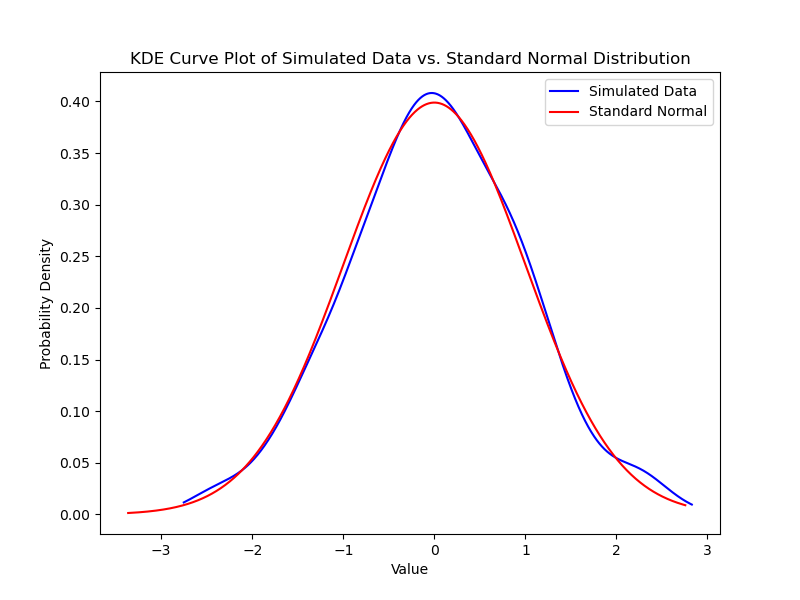
\includegraphics[width=\columnwidth]{2023/ST/57/codes/sim.png}
\caption{simulated vs standard normal }
\label{fig:57.2023/F/Fig1}
\end{figure}